\chapter{Proposta}\label{cap4}

\section{Usuários}


\section{Terminologias Existentes}

\subsection{Tesauros}

\subsection{Ontologias Existente}


\section{Descrição do Ambiente Web}


\section{Cronograma}
A criação das atividades desse cronograma foram baseadas no plano de ensino da disciplina Tópicos especiais em Engenharia de Software. Este plano foi desenvolvido para o primeiro semestre letivo no ano de 2015.

 \begin{figure}[ht]
  \centering
    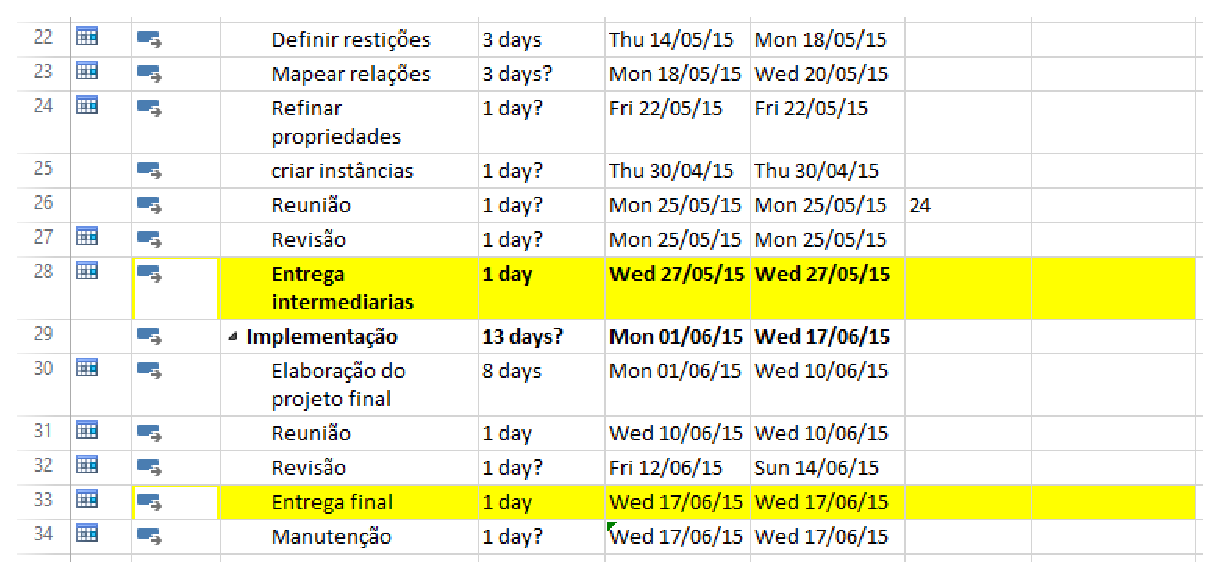
\includegraphics[keepaspectratio=true,scale=0.5]{figuras/cronograma.eps}
  \caption{Cronograma do projeto}
\end{figure}